\chapter{Computational learning theory}

\begin{description}
    \item[Instance space] \marginnote{Instance space}
        Set $X$ of (encoded) instances of objects that a learner wants to classify.

        Data from the instance space is drawn from a distribution $\mathcal{D}$ unknown to the learner.

    \item[Concept] \marginnote{Concept}
        Subset $c \subseteq X$ of the instance space which can be intended as properties of objects (i.e. a way to classify the instance space).

    \item[Concept class] \marginnote{Concept class}
        Collection $\mathcal{C} \subseteq \mathbb{P}(X)$ of concepts.

        It represents the concepts that are sufficiently simple for the algorithm to handle (i.e. the space of learnable concepts).

        \begin{description}
            \item[Target concept]
                Concept $c \in \mathcal{C}$ that the learner wants to learn.
        \end{description}

        \begin{remark}
            A learning algorithm is designed to learn concepts from a concept class
            neither knowing the target concept nor its data distribution.
        \end{remark}

    \item[Learning algorithm] \marginnote{Learning algorithm}
        Given a concept class $\mathcal{C}$ and a target concept $c \in \mathcal{C}$ with unknown distribution $\mathcal{D}$, 
        a learning algorithm $\mathcal{A}$ takes as input:
        \begin{itemize}
            \item $\varepsilon$, the error parameter (or accuracy if seen as $(1-\varepsilon)$),
            \item $\delta$, the confidence parameter,
            \item $EX(c, \mathcal{D})$, an oracle that $\mathcal{A}$ can call to retrieve a data point $x \sim \mathcal{D}$ 
                with a label to indicate whether it is in the target concept $c$ or not (i.e. training data),
        \end{itemize}
        and outputs a concept $h \in \mathcal{C}$. 
        \begin{center}
            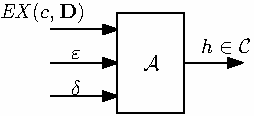
\includegraphics[width=0.3\linewidth]{./img/_learning_algorithm.pdf}
        \end{center}

        \begin{description}
            \item[Probability of error] \marginnote{Probability of error}
                Given a concept class $\mathcal{C}$, 
                a target concept $c \in \mathcal{C}$ with unknown distribution $\mathcal{D}$ and 
                a learning algorithm $\mathcal{A}$,
                the probability of error (i.e. misclassifications) for any output $h \in \mathcal{C}$ of $\mathcal{A}$ is defined as:
                \[ \text{error}_{\mathcal{D}, c} = \mathcal{P}_{x \sim \mathcal{D}}[ h(x) \neq c(x) ] \]
        \end{description}

        \begin{figure}[H]
            \centering
            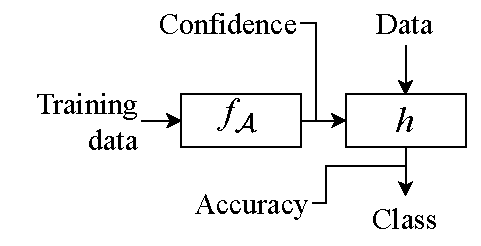
\includegraphics[width=0.35\linewidth]{./img/_learning_model.pdf}
            \caption{General idea of a learning algorithm $\mathcal{A}$ computed as a function $f_\mathcal{A}$}
        \end{figure}

    \item[PAC learnability] \marginnote{PAC learnability}
        A concept class $\mathcal{C}$ over the instance space $X$ is probably approximately correct (PAC) learnable iff there is an algorithm $\mathcal{A}$ such that:
        \begin{itemize}
            \item For each target concept $c \in \mathcal{C}$,
            \item For each distribution $\mathcal{D}$, 
            \item For each error $0 < \varepsilon < \frac{1}{2}$,
            \item For each confidence $0 < \delta < \frac{1}{2}$,
        \end{itemize}
        it holds that:
        \[ \mathcal{P}\left[ \text{error}_{\mathcal{D}, c}\Big( \mathcal{A}\big( EX(c, \mathcal{D}), \varepsilon, \delta \big) \Big) < \varepsilon \right] > 1-\delta \]
        where the probability is computed by sampling data points from $EX(c, \mathcal{D})$.

        In other words, the probability that $\mathcal{A}$ has an error rate lower than $\varepsilon$ (or an accuracy higher than $(1-\varepsilon)$) is greater than $(1-\delta)$.

        \begin{description}
            \item[Efficient PAC learnability] \marginnote{Efficient PAC learnability}
                A concept class $\mathcal{C}$ is efficiently PAC learnable iff
                it is PAC learnable and the algorithm $\mathcal{A}$ that learns it has 
                a time complexity bound to a polynomial in $\frac{1}{\varepsilon}$ and $\frac{1}{\delta}$.

                \begin{remark}
                    The complexity of $\mathcal{A}$ is measured taking into account the number of calls to $EX(c, \mathcal{D})$.
                \end{remark}
        \end{description}
\end{description}

\begin{example}[Axes-aligned rectangles in $\mathbb{R}^2_{[0, 1]}$]
    Consider the instance space $X = \mathbb{R}^2_{[0, 1]}$
    and the concept class $\mathcal{C}$ of concepts represented by all the points contained within a rectangle parallel to the axes of arbitrary size.

    \begin{figure}[H]
        \centering
        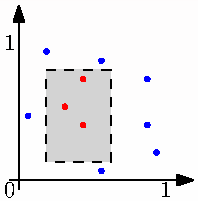
\includegraphics[width=0.2\linewidth]{./img/_learning_rectangle.pdf}
        \caption{Example of problem instance. The gray rectangle is the target concept, red dots are positive data points and blue dots are negative data points.}
    \end{figure}

    An algorithm has to guess a classifier (i.e. a rectangle) without knowing the target concept and the distribution of its training data.
    Let an algorithm $\mathcal{A}_\text{BFP}$ be defined as follows:
    \begin{itemize}
        \item Take as input some data $\{ ((x_1, y_1), p_1), \dots, ((x_n, y_n), p_n) \}$ where 
            $(x_i, y_i)$ are the coordinates of the point and $p_i$ indicates if the point is within the target rectangle.
        \item Return the smallest rectangle that includes all the positive instances.
    \end{itemize}

    Given the rectangle $R$ predicted by $\mathcal{A}_\text{BFP}$ and the target rectangle $T$,
    the probability of error in using $R$ in place of $T$ is:
    \[ \text{error}_{\mathcal{D}, T}(R) = \mathcal{P}_{x \sim \mathcal{D}} [ x \in (R \smallsetminus T) \cup (T \smallsetminus R) ] \]
    In other words, a point is misclassified if it is in $R$ but not in $T$ or vice versa.
    \begin{remark}
        By definition of $\mathcal{A}_\text{BFP}$, it always holds that $R \subseteq T$. 
        Therefore, $(R \smallsetminus T) = \varnothing$ and the error can be rewritten as:
        \[ \text{error}_{\mathcal{D}, T}(R) = \mathcal{P}_{x \sim \mathcal{D}} [ x \in (T \smallsetminus R) ] \]
    \end{remark}


    \begin{theorem}[Axes-aligned rectangles in $\mathbb{R}^2_{[0, 1]}$ PAC learnability]
        It holds that:
        \begin{itemize}
            \item For every distribution $\mathcal{D}$,
            \item For every error $0 < \varepsilon < \frac{1}{2}$, 
            \item For every confidence $0 < \delta < \frac{1}{2}$,
        \end{itemize} 
        if $m \geq \frac{4}{\varepsilon}\ln\left( \frac{4}{\delta} \right)$, then:
        \[ 
            \mathcal{P}_{D \sim \mathcal{D}^m}
                \left[ \text{error}_{\mathcal{D}, T}\Big( \mathcal{A}_\text{BFP}\big(T(D)\big) \Big) < \varepsilon \right]  > 1 - \delta
        \]
        where $D \sim \mathcal{D}^m$ is a sample of $m$ data points (i.e. training data)
        and $T(\cdot)$ labels the input data wrt to the target rectangle $T$.

        \begin{proof}
            By definition, the error of $\mathcal{A}_\text{BFP}$ is defined as:
            \[ \text{error}_{\mathcal{D}, T}(R) = \mathcal{P}_{x \sim \mathcal{D}} [ x \in (T \smallsetminus R) ] \]

            Consider the space defined by $(T \smallsetminus R)$ divided in four sections $E_1 \cup \dots \cup E_4 = (T \smallsetminus R)$:
            \begin{figure}[H]
                \centering
                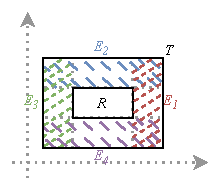
\includegraphics[width=0.4\linewidth]{./img/_rectangle_space.pdf}
            \end{figure}

            Consider the probabilistic event "$x \in E_i$".
            For the training data $x \sim \mathcal{D}$ this holds iff none of those points
            end up in $E_i$ as, if a training point is in $E_i$, $R$ would be bigger to include it and $E_i$ would be smaller.

            Now consider four other regions $F_1, \dots, F_4$ of the plane related to $E_i$ but defined differently
            in such a way that $\mathcal{P}_{x \sim D}[x \in F_i] = \frac{\varepsilon}{4}$.
            This can be achieved by expanding the $E_i$ regions to take some area of the rectangle $R$.
            \begin{figure}[H]
                \centering
                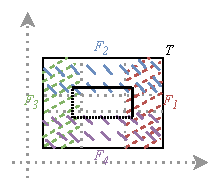
\includegraphics[width=0.4\linewidth]{./img/_rectangle_space2.pdf}
            \end{figure}

            Then, as $E_i$ are smaller than $F_i$, it holds that:
            \[ 
                \begin{split}
                    \mathcal{P}_{x \sim D}[x \in E_i] < \frac{\varepsilon}{4} &\Rightarrow \mathcal{P}_{x \sim D}[x \in (T \smallsetminus R)] < \varepsilon \\
                    & \Rightarrow \text{error}_{\mathcal{D}, T}(R) < \varepsilon
                \end{split}
            \]
            
            \textit{To be continued\dots}
        \end{proof}
    \end{theorem}
\end{example}
